\chapter{CellTAN: Cellular Time Activation Networks} \label{chap:chap4}

Distributed information systems characterized by time series data present various challenges, primarily due to their complex and dynamic nature. The sheer volume of data that must be processed and analyzed in real time is a significant challenge, leading to concerns over storage, computation, and scalability. Moreover, data quality issues such as missing or incomplete data and data heterogeneity arising from sourcing data from disparate sources with varying consistency and structure further exacerbate these challenges. Another critical challenge of these systems is handling the temporal aspects of time series data, requiring specialized pre-processing, feature extraction, and modeling techniques. The distributed nature of these systems further complexifies matters, with issues encompassing data synchronization and accuracy being a common concern. Furthermore, their implementation in real-world applications requires robust mechanisms for data security and privacy, which adds a layer of complexity to the design and implementation of these systems.

\begin{figure}[h]
    \centering
    \includegraphics[width=10cm]{figures/chapter4/cell/celltan.pdf}
    \caption{Ilustrative overview of a CellTAN.}
    \label{fig:celltan}
\end{figure}

This chapter proposes a novel tool entitled CellTAN (Cellular Time Activation Network) to address such challenges. CellTAN represents sparse yet interconnected components that function independently, cooperatively, and asynchronously.
Inspired by other effective mechanisms like GNNs, CXNs, and Weighted Cross-Connection Networks (WCCNs), CellTAN uses a graph-like structure to represent a network of components. Following the introductory chapters, its primary purpose is to detect anomalous scenarios on PV systems. However, its generalized formulation introduces other valuable features which come naturally from fulfilling this goal. Such are state estimation, forecasting, and PV operator collaboration (while maintaining data privacy). For briefness' sake, future sections will highlight the other benefits of CellTAN.

Instead of tackling fault detection and classification in a classical centralized manner, which is already extensively showcased throughout the literature, this tool approaches the same problem with a paradigm change: a distributed system. By having a virtual representation closely related to the physical form of the system, relationships between components can be leveraged to assess their correct (or incorrect) operation. While initially designed for photovoltaic (PV) systems, the concepts of cells, connections, neighbors, time series, and uncertainty are universal and applicable to other fields such as biology, physics, and more. The potential for generic applicability sparks the interest to not bake specifics of PV systems directly into this tool so that its preserved from usage with other distributed systems.

% escrever sobre os benefícios?

Figure \ref{fig:celltan} illustrates a simple CellTAN network overview. Regarding the \textbf{Hub}, one might infer (correctly) that it breaks the non-centralized paradigm. Nevertheless, it is present to solve some real-life implementation challenges and limitations, as will be further discussed in this chapter. The subsequent sections explain the working of the \textbf{Cell} and its interactions within the network. Since it is the core component, understanding its behavior is crucial for a complete understanding of the tool.

\section{Glossary}

\begin{itemize}
    \item \textbf{Knowledge base}: refers to registered historical knowledge (samples) of time series variables.
    
    \item \textbf{Inputs}: a set of variables that define the state of a cell. Instantaneous values, represented by uniform fuzzy numbers.

    \item \textbf{Outputs}: similar to inputs, but obtained through certain computations.

    \item \textbf{Time decay}: a process associated with increased uncertainty of variables over time.
    
    \item \textbf{Time Activations}: timestamps of past ocurrences that have a non zero value of membership against the sets of recent inputs.

    \item \textbf{Hub}: the central component of the cell network, which facilitates its visualization, management, and expansion. It acts as the proxy agent between the cell's communication.
    
\end{itemize}

\section{The Cell}

A cell is an independent entity composed of \textbf{data} and \textbf{processes}. As an individual part of the system, it follows a set of rules that define its intrinsic and extrinsic behavior. These rules address data privacy, request boundaries, and real-world operational limitations.

\paragraph*{Independence} During operation, independence on neighbors or other network entities for continuous processing of outputs results in a more robust system and increases availability. Thus, the cell shall be unbothered of its surroundings and continue operating in an isolated state given any connection cutoffs. This, of course, is not its preferred state, but enduring isolation until outside contact is re-established avoids shutdown and startup procedures. 

\paragraph*{Selfish Computations} The cell is selfish in that it will not perform any computations based on the request of others. This aspect creates a fundamental layer of protection against overloading the infrastructure in which it is deployed, which also increases availability.

\paragraph*{Selfless Data} Although selfish in computations, the cell shall provide access to a select set of data useful to the network. However, public data shall not compromise the cell's privacy (more on this later).

\subsection{Cell's Core}

\subsubsection{Temporal similarity extraction}

Temporal similarity extraction the process of identifying recurring patterns in time series data. It involves the identification of past instances where the current state is observed to extract useful information about the system's behavior over time. By identifying historical periods with similar states, temporal similarity extraction can help assess the current state or predict future trends. This technique is common in statistics, for purposes such as estimation and forecasting. Nonetheless, the process of temporal similarity extraction can be challenging due to the complexity and size of time series data, as well as the need to accurately measure and compare similarity across different periods.

% One approach to simplifying the process of temporal similarity extraction in multi-variate time series data is to use classical or fuzzy sets to filter historical data. This technique involves assigning a membership to each data point in the time series based on the corresponding set generated from the current cell inputs. Using sets, especially fuzzy ones, to represent inputs can capture the inherent uncertainty in time series data, making the approach more robust to noisy or incomplete data. We use classical sets as a starting point since filtering history becomes trivial and efficiently performed: constrain the knowledge base to samples where all variables belong to a corresponding interval. However, this simplification does not account for density since the filter reflects a binary state: a value either belongs to the uniform interval defined by the set (membership equals one) or doesn't (membership equals zero). This decision was taken to lighten the computational load in the cell's core for historical filtering since it equates to a simple bounded filter on each time series variable. Nonetheless, adequate fuzzy sets or probability distributions could result in more accurate temporal similarity extraction if it closely relates to the variable's statistical data.

Using sets or probability distributions to filter historical data is one approach to simplify the process of temporal similarity extraction in multivariate time series data. This approach assigns membership values to each data point in the time series based on the corresponding set (or distribution) generated from the current cell inputs. Representing inputs this way can better capture the inherent uncertainty in time series data, making the approach relatively robust to noisy or incomplete data. The proposal for similarity extraction in the cell consists of receiving crisp, updated values for the cell's variables from a data source (sensors or other data acquisition equipment, calculations, forecasting, etc.), generating a classical set, fuzzy number, or probability distribution from the crisp value can follow the following:

\begin{itemize}
    \item Classical set: simple uncertainty band (e.g. uncertainty up, down, relative, etc);
    \item Fuzzy number: generalized fuzzy number representation \cite{Zhang2019} (e.g. triangular fuzzy number (a,b,d;h));
    \item Probability distribution: the distribution's characteristics (e.g. mean ($\mu$) and standard deviation ($\delta$) for Gaussian, mean rate of occurence ($\lambda$) for Poisson, etc.);
\end{itemize}

The initial choice is to use classical sets since filtering history becomes trivial and efficient: restrict the knowledge base to samples where all variables belong to a corresponding interval. From now on, equations refering to the time variable $t$ assumes that present time is equal to $t=0$ and membership functions are represented by $\mu$.

% A célula podia aceitar em cada valor se queria um numero fuzzy e ter mais que um disponivel ou aceitar distribuição probabilística.

\paragraph{Self Similarity}

With a knowledge base and input variables, the cell can perform intrinsic temporal similarity extraction. When filtering historical data with two or more variables, there should be a trend of narrowing down the resulting data, which can be utilized to construct outputs with equal or less uncertainty.

To demonstrate this process, consider the a cell that is characterized by two variables, which are a function of time: $x(t)$ and $y(t)$. 
Assume that, at a given instant, these are the new cell inputs:

\begin{equation}
x(0) = 1.0 \rightarrow \mu_{x(0)}(x) =
\begin{cases}
1, & x \in [0.9, 1.1] \\
0, & x \notin [0.9, 1.1] \\
\end{cases}
\end{equation}

\begin{equation}
y(0) = 2.0 \rightarrow \mu_{y(0)}(y) =
\begin{cases}
1, & y \in [1.8, 2.2] \\
0, & y \notin [1.8, 2.2] \\
\end{cases}
\end{equation}

\begin{figure}[h!]
    \centering
    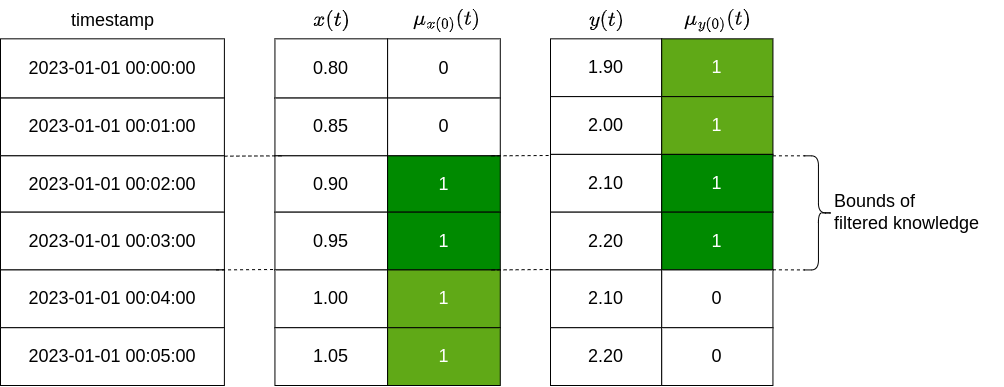
\includegraphics[width=\linewidth]{figures/chapter4/cell/solo_state_estimation.drawio.png}
    \caption{Visualization of a self similarity extraction example.}
    \label{fig:solo_state_estimation}
\end{figure}

Considering the knowledge base represented in figure \ref{fig:solo_state_estimation}, we can observe that the resulting activations will be 2023-01-01 00:02:00 and 2023-01-01 00:03:00. These are the timestamps of past instances where the cell's variables have values belonging to the set generated from new inputs. We can also infer that the values of $x$ and $y$ should reside in a set constrained by the filtered historical values ($x(t)$ and $y(t)$). The outputs based on self similarity extraction are:

\begin{equation}
    x'(0) \in [0.90, 0.95]
\end{equation}

\begin{equation}
    y'(0) \in [1.80, 2.20]
\end{equation}

\paragraph{Mutual Similarity}
Capacidade de estimação de estado intrínsica + extrínsica

\subsection{Connections and Trust}
O que é uma conexão, como se caracteriza, e que valores tem a ela associada
